\documentclass[11pt]{article}
\usepackage{latexsym}
\usepackage{amsmath}
\usepackage{amssymb}
\usepackage{amsthm}
\usepackage{epsfig}
\usepackage[tight]{subfigure}
\usepackage{todonotes} % for comments
\usepackage{float}

\usepackage{amsmath,amssymb}
\usepackage{scrextend}

\DeclareMathOperator*{\minimize}{min}
\DeclareMathOperator*{\maximize}{max}

\usepackage{algorithm}
 %on linux you may need to run sudo apt-get install texlive-full to install algorithm.sys
\usepackage{algorithmic}

\usepackage{verbatim}

\newcommand{\handout}[5]{
  \noindent
  \begin{center}
  \framebox{
    \vbox{
      \hbox to 5.78in { {#1} \hfill #2 }
      \vspace{4mm}
      \hbox to 5.78in { {\Large \hfill #5  \hfill} }
      \vspace{2mm}
      \hbox to 5.78in { {\em #3 \hfill #4} }
    }
  }
  \end{center}
  \vspace*{4mm}
}

\newcommand{\lecture}[5]{\handout{#1}{#2}{#3}{#4}{#5}}
\newcommand{\collision}[0]{\mathrm{collision}}
\newcommand{\nocollision}[0]{\overline{\collision}}

\newcommand{\argmin}[1]{\underset{#1}{\operatorname{arg}\,\operatorname{min}}\;}
\newcommand*{\QED}{\hfill\ensuremath{\square}}

\newtheorem{theorem}{Theorem}
\newtheorem{corollary}[theorem]{Corollary}
\newtheorem{lemma}[theorem]{Lemma}
\newtheorem{observation}[theorem]{Observation}
\newtheorem{proposition}[theorem]{Proposition}
\newtheorem{definition}[theorem]{Definition}
\newtheorem{claim}[theorem]{Claim}
\newtheorem{fact}[theorem]{Fact}
\newtheorem{assumption}[theorem]{Assumption}
\newtheorem{note}[theorem]{Note}

% 1-inch margins, from fullpage.sty by H.Partl, Version 2, Dec. 15, 1988.
\topmargin 0pt
\advance \topmargin by -\headheight
\advance \topmargin by -\headsep
\textheight 8.9in
\oddsidemargin 0pt
\evensidemargin \oddsidemargin
\marginparwidth 0.5in
\textwidth 6.5in

\parindent 0in
\parskip 1.5ex
%\renewcommand{\baselinestretch}{1.25}

\begin{document}

\lecture{Statistical Techniques in Robotics (16-831, S22)}{Lecture \#07
  (Wednesday, February 9)}{Lecturer: Kris Kitani}{Scribes: Grace Brueggman, Yuqing Qin}{Follow the Regularized Leader}

\section{Review}
\subsection{Follow the Leader (FTL)}
In the previous lecture, we introduced the online convex optimization problem as a generalized version of online learning and the "Follow the Leader" (FTL) algorithm. FTL algorithm is a generic online optimization algorithm that follows two main steps. The first step is to estimate the parameters $\bm{w}$ such that it could minimize the cumulative loss up to time $t-1$. After the prediction step, it is going to receive the new loss function that will be used in the next timestamp. The algorithm is summarized below in Algorithm \ref{algo:FTL}.

%Length requirement 1-2 pages.
\begin{algorithm}[H]
\caption{Follow the Leader}
\label{algo:FTL}
\begin{algorithmic}[1]

\FOR{$t=1, 2,\,\cdots,\;T$}
    \STATE $\bm{w}^{(t)}$ = $\argmin{\bm{w} \in W} \sum^{t-1}_{i=1} f^{(i)} (\bm{w})$ \hfill $\triangleright$ Parameter estimation
    \STATE \textsc{Receive} ($f^{(t)} : W \rightarrow \mathbb{R}$) \hfill $\triangleright$ Update loss function
\ENDFOR

\end{algorithmic}
\end{algorithm}

We also saw two examples of FTL algorithm by applying different loss functions. With simple linear loss function as defined below, we saw it failed with the regret growing linearly. 

\begin{equation*}
    f^{(t)} (w) = wz^{(z)}
\end{equation*}

The total loss of the FTL learner using the linear loss function is linearly to the time, and as a result, the regret also grows linearly. 

\begin{equation*}
    L = \sum_{t=1}^T f^{(t)} = \sum_{t=2}^T 1 = T -1
\end{equation*}

\begin{equation*}
    Regret(\bm{u}) = T -1 = O(T)
\end{equation*}

To further improve the performance, we also define a quadratic loss function, which in turn gives us lower regret bound. The quadratic loss is defined as below:

\begin{equation*}
    f^{(t)} (w) = \frac{1}{2}||\bm{w} - \bm{z}^{(t)}||_2^2
\end{equation*}

The regret bound for FTL with above quadratic loss function is better than the linear loss function's, which gives us a no regret algorithm.

\begin{equation*}
    Regret \leq 4L^2 (log(T) + 1) = O(logT)
\end{equation*}

In today's lecture, we will show the proof of this better regret bound given by FTL with quadratic loss function and try to modify the linear loss function to make it perform better.

\section{Summary}
\subsection{FTL with Quadratic Loss}
The quadratic loss is defined as below:

\begin{equation*}
    f^{(t)} (w) = \frac{1}{2}||\bm{w} - \bm{z}^{(t)}||_2^2
\end{equation*}

We also assume 

\begin{equation*}
    ||z||_2^2 \leq L
\end{equation*}


\begin{algorithm}[H]
\caption{Follow the Leader with Quadratic Loss}
\label{algo:FTL_Q}
\begin{algorithmic}[1]

\FOR{$t=1, 2,\,\cdots,\;T$}
    \STATE $\bm{w}^{(t)}$ = $\argmin{\bm{w} \in W} \sum^{t-1}_{i=1} f^{(i)} (\bm{w})$ \hfill $\triangleright$ Parameter estimation
    \STATE \textsc{Receive} ($f^{(t)} (w) = \frac{1}{2}||\bm{w} - \bm{z}^{(t)}||_2^2$) \hfill $\triangleright$ Quadratic loss function
\ENDFOR

\end{algorithmic}
\end{algorithm}

From the quadratic loss definition, we could minimize the loss by taking the derivatives of it and obtain the optimal $\bm{w}$. The minimizer of a sum of squared difference is the average over the elements. As a result, we could rewrite line 2 in above algorithm to be:

\begin{equation*}
    \bm{w}^{(t)} = \frac{1}{t-1} \sum_{i=1}^{t-1}z^{(i)}
\end{equation*}

\subsubsection{Regret Bound}
The regret bound for FTL with quadratic loss is 

\begin{equation*}
    Regret \leq 4L^2 (log(T) + 1)
\end{equation*}

To derive this regret bound, we use a new proof technique with only two steps. 

\begin{itemize}
    \item Upper-bound the regret using the one-step look ahead cheater
    \item Approximations and Algebra
\end{itemize}

By definition, the cumulative regret is defined as 

\begin{equation*}
    R(u) = \sum_t [f^{(t)} (w^{(t)}) - f^{(t)}(u)]
\end{equation*}

The first term in this regret equation represents the loss of the online learner, and the second term is the loss of some hypothesis $u$

The best hypothesis at timestamp $t$ is actually the one that could minimize the cumulative loss up to time $t$. Therefore,

\begin{equation*}
    Best Hypothesis = \argmin w \sum_{i=1}^t f^{(i)} = \bm{w}^{(t+1)}
\end{equation*}

The best hypothesis at time $t$ is the next time step's parameter $w^{(t+1)}$. We called this "one step look ahead cheater". With this, we could derive the regret bound as below:

\begin{equation*}
    R(u) = \sum_t [f^{(t)} (w^{(t)}) - f^{(t)}(u)] \leq \sum_t [f^{(t)} (w^{(t)}) - f^{(t)}(\bm{w}^{(t+1)})]
\end{equation*}

To prove this regret bound, we only need to prove:

\begin{equation*}
   \sum_{t=1}^T [ f^{(t)}(w^{(t+1)})] \leq \sum_{t=1}^T [f^{(t)} (u) ]
\end{equation*}

Proof by Induction is to assume claim for T-1 and prove it holds for T. We will use this strategy to prove the above. Therefore, we take one step before, and assume

\begin{equation*}
   \sum_{t=1}^{T-1} [ f^{(t)}(w^{(t+1)})] \leq \sum_{t=1}^{T-1} [f^{(t)} (u) ]
\end{equation*}

When we add $f^{(T)}(w^{(T+1)})$ at time step $T$ to both sides, we could get

\begin{equation*}
   \sum_{t=1}^{T} [ f^{(t)}(w^{(t+1)})] \leq f^{(T)}(w^{(T+1)}) + \sum_{t=1}^{T-1} [f^{(t)} (u) ]
\end{equation*}

The left hand side gets absorb the time step $T$'s loss, but the right hand side could not simply absorb that new loss term. Since the inequality holds for all values of $u$, and we can make the right hand side to be simpler by making the $u = w^{(T+1)}$. Therefore,

\begin{equation*}
   \sum_{t=1}^{T} [ f^{(t)}(w^{(t+1)})] \leq \sum_{t=1}^{T} [f^{(t)} (w^{(T+1)}) ]
\end{equation*}

The only difference between the left hand side and the right hand side is on the $w^{(T+1)}$, the left hand side means we always use one step look ahead cheater (difference cheaters at each time step), the right hand side means we only use one single cheater (the cheater at the end of the sequence) for all time steps.

The minimizer by definition,

\begin{equation*}
    \bm{w}^{(T+1)} = \argmin u \sum_{t=1}^T f^{(t)} (u) \leq u
\end{equation*}

Therefore, the above cumulative loss inequality's RHS can be upper bounded by all $u$, which is

\begin{equation*}
   \sum_{t=1}^{T} [ f^{(t)}(w^{(t+1)})] \leq \sum_{t=1}^{T} [f^{(t)} (u) ]
\end{equation*}

We have successfully proved the regret inequality without making any assumption yet. The regret bound is

\begin{equation*}
    R(u) = \sum_t [f^{(t)} (w^{(t)}) - f^{(t)}(u)] \leq \sum_t [f^{(t)} (w^{(t)}) - f^{(t)}(\bm{w}^{(t+1)})]
\end{equation*}

Now, we will assume the loss function is quadratic, insert the loss into the RHS of the bound,

\begin{equation*}
    f^{(t)} (w^{(t)}) - f^{(t)}(\bm{w}^{(t+1)}) = \frac{1}{2}||\bm{w}^{(t)} - \bm{z}^{(t)}||_2^2 - \frac{1}{2}||\bm{w}^{(t+1)} - \bm{z}^{(t)}||_2^2
\end{equation*}

To further simply this, we could rewrite the weight update into an incremental form. Recall that the minimizer of quadratic loss function is just the average. Instead of taking the average over all the values for each time step, we could simply incrementally add the new value with the previous mean value and normalize it. Therefore,

\begin{equation*}
    \bm{w}^{(t+1)} = (1- \frac{1}{t})w^{(t)} + ( \frac{1}{t}) z^{(t)}
\end{equation*}

To plug it in the regret bound,

\begin{equation*}
    f^{(t)} (w^{(t)}) - f^{(t)}(\bm{w}^{(t+1)}) = \frac{1}{2}||\bm{w}^{(t)} - \bm{z}^{(t)}||_2^2 - \frac{1}{2}||(1- \frac{1}{t})w^{(t)} + ( \frac{1}{t}) z^{(t)} - \bm{z}^{(t)}||_2^2
\end{equation*}

\begin{equation*}
    = \frac{1}{2}(1-(1-\frac{1}{t})^2)||w^{(t)} - z^{(z)}||_2^2
\end{equation*}

In the graph at Figure \ref{fig:ftrl_examples} we depict two functions.

\begin{center}
(1) $f(t) = \frac{1}{t}$

(2) $f(t) = \frac{1}{2}(1-(1-\frac{1}{t})^2)$
\end{center}

\begin{figure}[h]
    \centering
    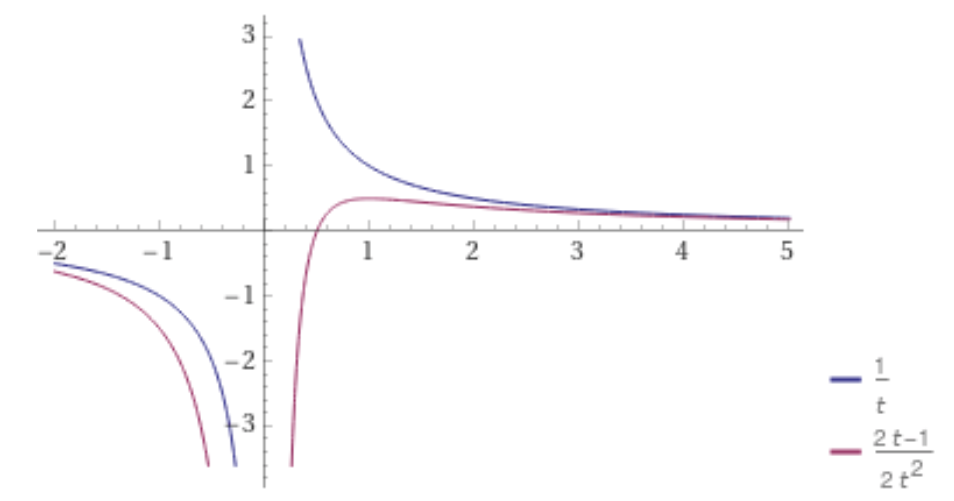
\includegraphics[width=0.5\textwidth]{figures/quadratic.png}
    \caption{The known inequality}
    \label{fig:ftrl_examples}
\end{figure}

Because of the relationship between these functions, where we can create the following inequality:
\begin{center}
$\frac{1}{2}(1-(1-\frac{1}{t})^2) \leq \frac{1}{t}$
\end{center}

With this inequality, we can derive the upper bound for the FTL regret.

\begin{equation*}
    \frac{1}{2}(1-(1-\frac{1}{t})^2)||w^{(t)} - z^{(z)}||_2^2 \leq \frac{1}{t}||w^{(t)} - z^{(z)}||_2^2
\end{equation*}

Recall that we made prior assumptions that

\begin{equation*}
    L = max_t ||z^{(t)}||
\end{equation*}

Since the average is always less or equal to the max,

\begin{equation*}
    ||w^{(t)}|| \leq L
\end{equation*}

From this, we could derive below inequality based on the triangle inequality. We could think of two vectors, each might have a magnitude of $L$, therefore, 

\begin{equation*}
   ||w^{(t)} - z^{(t)}|| \leq 2L
\end{equation*}

As a result, the regret at time $t$ is upper bounded by
\begin{equation*}
    \frac{1}{2}(1-(1-\frac{1}{t})^2)||w^{(t)} - z^{(z)}||_2^2 \leq \frac{1}{t}||w^{(t)} - z^{(z)}||_2^2 \leq (\frac{1}{t}) 4L^2
\end{equation*}

The regret bound over all time steps is

\begin{equation*}
    R(u) \leq \sum_t [f^{(t)} (w^{(t)}) - f^{(t)}(\bm{w}^{(t+1)})] \leq \sum_t (\frac{1}{t}) 4L^2
\end{equation*}


Another useful inequality to simply this is

\begin{equation*}
     \sum_{t=1}^T (\frac{1}{t}) \leq log(T) + 1
\end{equation*}

Plug it in and we can get the final regret bound,

\begin{equation*}
    R(u) \leq 4L^2(log(T) + 1)
\end{equation*}

To summarize the FTL with quadratic loss function, we could see the algorithm is a no regret algorithm from the above regret bound. Also the weight update is via averaging, which updates the weights smoothly. The weight does not change dramatically over time and it ensure the stability for the algorithm.


\subsection{Follow the Regularized Leader (FTRL)}
The generic  version of the Follow the Regularized Leader is just like FTL with a regularizer term added in the parameter estimation. We can even think of FTL as a special case of FTRL where $\psi = 0$. In Algorithm \ref{algo:FTRL} below, S is a convex set.

\begin{algorithm}[H]
\caption{Follow the Regularized Leader}
\label{algo:FTRL}
\begin{algorithmic}[1]
\FOR{$t=1, 2,\,\cdots,\;T$}
    \STATE $\bm{w}^{(t)}$ = $\argmin{\bm{w}} \sum^{t-1}_{i=1} f^{(i)} (\bm{w}) + \psi (\bm{w})$ \hfill $\triangleright$ Parameter estimation
    \STATE \textsc{Receive} ($f^{(t)} : S \rightarrow \mathbb{R}$) \hfill $\triangleright$ Update loss function
\ENDFOR

\end{algorithmic}
\end{algorithm}


\subsubsection{Follow the Regularized Leader (FTRL) with Linear Loss and Quadratic Regularization}

One way to structure FTRL is with quadratic regularization and linear loss. With quadratic regularization, we use the following to calculate $\psi(\bm{w})$, such that the regularizer is minimized when the parameters $\mb{w} = 0$ and it induces an exponential penalty when the parameters are large:
\[
\psi(\bm{w}) = \frac{1}{2\eta}||\bm{w}||^2_2
\]
To calculate a linear loss, we use the function:
\[
f^{(t)} = \bm{w}\cdot\bm{z}^{(t)}
\]
As with all losses, it is a more optimized online learner solution when we minimize this term incrementally.

\begin{algorithm}[H]
\caption{Follow the Regularized Leader with Quadratic Regularization and Linear Loss}
\label{algo:FTRL_quadR_linL}
\begin{algorithmic}[1]

\FOR{$t=1, 2,\,\cdots,\;T$}
    \STATE $\bm{w}^{(t)}$ = $\argmin{\bm{w} \in S} (\frac{1}{2\eta}||\bm{w}||^2_2 + \bm{w}\cdot\sum^{t-1}_{i=1} \bm{z}^{(i)})$ \hfill $\triangleright$ Parameter estimation
    \STATE \textsc{Receive} ($f^{(t)}(\bm{w}) = \bm{w}\cdot\bm{z}^{(t)}$ \hfill $\triangleright$ Update loss function
\ENDFOR

\end{algorithmic}
\end{algorithm}

To find the minimum of the parameter estimation step in Algorithm \ref{algo:FTRL_quadR_linL}, we have to first take the derivative of the cumulative loss with respect to $\bm{w}$ and then solve for $\bm{w}$.
\begin{equation*}
\frac{d}{dw}(\frac{1}{2\eta}||\bm{w}||^2_2 + \bm{w}\cdot\sum^{t-1}_{i=1} \bm{z}^{(i)}) = 0
\end{equation*}
\begin{equation*}
\frac{1}{2\eta}2\bm{w} + \sum^{t-1}_{i=1} \bm{z}^{(i)} = 0
\end{equation*}
\begin{equation*}
\bm{w}^{(t)} = -\eta \sum^{t-1}_{i=1} \bm{z}^{(i)}
\end{equation*}

Another way to look at $\bm{w}$ is in a recursive form where the new parameter is in terms of the old parameter and the incremental update is proportional to the gradient of the loss function at t, $\bm{z}^{(t-1)}$, such that:
\begin{equation*}
\bm{w}^{(t)} =  -\eta (\sum^{t-2}_{i=1} \bm{z}^{(i)} + \bm{z}^{(t-1)})
\end{equation*}
\begin{equation*}
\bm{w}^{(t)} =  -\eta \sum^{t-2}_{i=1} \bm{z}^{(i)} - \eta \bm{z}^{(t-1)}
\end{equation*}
\begin{equation*}
\bm{w}^{(t)} =  \bm{w}^{(t-1)} - \eta \bm{z}^{(t-1)}
\end{equation*}

\subsubsection{Regret Bound for FTRL with a Euclidean Regularizer and Linear Loss}
\textbf{Proof of Regret Bound}:
\begin{equation*}
R^{(T)}(\bm{u}) \leq [\psi(\bm{u}) - \psi(\bm{w}^{(1)})] + \sum^{T}_{t=1}[f^{(t)}(\bm{w}^{(t)}) - f^{(t)}(\bm{w}^{(t+1)})]
\end{equation*}
We then substitute in definitions. We also set $\psi(\bm{w}^{(1)}) = 0$, since we know $\bm{w}^{(1)}$ is the argmin of the L2 norm regularizer, which we previously determined is minimized at 0.
\begin{equation*}
= [\frac{1}{2\eta}||\bm{u}||^2_2 - 0] + \sum^{T}_{t=1}[<\bm{w}^{(t)}, \bm{z}^{(t)}> - <\bm{w}^{(t+1)}, \bm{z}^{(t)}>]
\end{equation*}
\begin{equation*}
= \frac{1}{2\eta}||\bm{u}||^2_2 + \sum^{T}_{t=1}[<\bm{w}^{(t)} - \bm{w}^{(t+1)}, \bm{z}^{(t)}> ]
\end{equation*}

Given the recursive form for the update parameter step derived above in Section 2.2.1, we know:
\begin{equation*}
\bm{w}^{(t+1)} = \bm{w}^{(t)} - \eta\bm{z}^{(t)}
\end{equation*}
\begin{equation*}
\bm{w}^{(t)} - \bm{w}^{(t+1)} = \eta\bm{z}^{(t)}
\end{equation*}
which can now be substituted into the following:
\begin{equation*}
R^{(T)}(\bm{u}) \leq \frac{1}{2\eta}||\bm{u}||^2_2 + \sum^{T}_{t=1}\eta||\bm{z}^{(t)}||^2
 \end{equation*}
Since this is the upper bound, we will establish the following:
\begin{equation*}
L = max_{\bm{z}}||\bm{z}||_2
\end{equation*}
\begin{equation*}
B = max_{\bm{u} \in S}||\bm{u}||_2
\end{equation*}
Which, when substituted into the inequality, we have the cleaner solution:
\begin{equation*}
R^{(T)}(\bm{u}) \leq \frac{1}{2\eta}B^2 + \eta TL^2
\end{equation*}
The optimal $\eta$ can be determined by taking the derivative of the RHS with respect to $\eta$ and solving for $\eta$.
\begin{equation*}
\frac{d}{d\eta}( \frac{1}{2\eta}B^2 + \eta TL^2) = 0
\end{equation*}
\begin{equation*}
-\frac{1}{2\eta^2}B^2 + TL^2 = 0
\end{equation*}
\begin{equation*}
\frac{2TL^2}{B^2}  = \frac{1}{\eta^2}
\end{equation*}
\begin{equation*}
\frac{B^2}{2TL^2}  = \eta^2
\end{equation*}
\begin{equation*}
\frac{B}{L\sqrt{2T}}  = \eta
\end{equation*}
We then take this this value of $\eta$ and put it in the inequality to get the upper bound of the regret:
\begin{equation*}
R^{(T)}(\bm{u}) \leq \frac{1}{2(\frac{B}{L\sqrt{2T}})}B^2 +  (\frac{B}{L\sqrt{2T}}) TL^2
\end{equation*}
\begin{equation*}
R^{(T)}(\bm{u}) \leq BL\sqrt{2T}
\end{equation*}
This means FLRL with a linear loss and quadratic regularization is a no regret algorithm, or more explicitly,  over a long time, the average regret will go to zero.

In relation to Convex Optimization, any sequence of Lipschitz loss functions, not just linear, and any convex regularization, not just quadratic, will also achieve stabilized results.
%\section*{References}
%Include your references here. Please cite any resources you found useful.	
%Populate the refs.bib file or list your references manually. Be consistent in formatting!
% {
% \bibliography{refs}
% \bibliographystyle{abbrv}
% }

% \section{Appendix}

%This section provides any relevant background material that was not covered in the lectures, but was found to be useful for understanding the material. 
%For example, derivations, theory underlying techniques employed, etc. 

%Additionally, this section can summarizes applications or extensions of these techniques found in the literature. 


\end{document} % Done!


